% \documentclass[review]{siamonline1116}
\documentclass{article}
% \usepackage{geometry} % see geometry.pdf on how to lay out the page. There's lots.
% \usepackage{hyperref}
\usepackage{graphicx}
\usepackage{gensymb}
% \usepackage[affil-it]{authblk}
% \usepackage[toc,page]{appendix}
% \usepackage{pifont}
\usepackage{amsmath}
% \usepackage{amsthm}
\usepackage{amsfonts}
\usepackage{hyperref}
\usepackage{cleveref}

% \usepackage{float}

\newtheorem{theorem}{Theorem}
\newtheorem{corollary}{Corollary}
\newtheorem{lemma}{Lemma}

\newcommand\numberthis{\addtocounter{equation}{1}\tag{\theequation}}

\renewcommand{\vec}[1]{\mathbf{#1}}

% \usepackage{draftwatermark}



% \SetWatermarkText{DRAFT}
% \SetWatermarkScale{6}
% \SetWatermarkLightness{0.95}

% \geometry{letter} % or letter or a5paper or ... etc
% \geometry{landscape} % rotated page geometry

% See the ``Article customise'' template for come common customisations

\title{A Ferrofluid Check-valve}
\author{Robert L. Read \\
    Founder, Public Invention \\
    Austin, TX, 78704 \\
    Email: \href{mailto:read.robert@gmail.com}{read.robert@gmail.com} 
}



\date{\today}

%%% BEGIN DOCUMENT
\begin{document}

\maketitle

%% TODO: Add something about Tetrobots into abstract.
\begin{abstract}
  A simple design for a ferrofluid check valve (one-way valve) is
  presented.
\end{abstract}


\section{Introduction}

It is relatively easy to make a ferrofluid piston. By making
a ferrofluid check valve, it becomes possible to make a pump
whose only moving parts are ferrofluid.  Such a pump can
be used to build a variety of actuators.

\section{Principle}

The key insight of the ferrofluid check valve is that a bubble inside a
a blob of ferrofluid with a magnetic flux gradient will move away from
the region of greater magnetic flux toward the region of less magnetic
flux. The viscoscity and ``hardness'' of ferrofluid increases
with magnetic flux.

Increasing air pressure on a blob of ferrofluid inside a magnetic
field tends to push the whole blob.

Because of this fundamental anisotropy, it is possible to
create a one-way valve.

If you build a physical structure in which air moving one way
pushes the whole blob and moving the other way is injected inside
the blob, then you have in theory created a one-way valve.

%% \begin{figure}
%%   \centering
%%      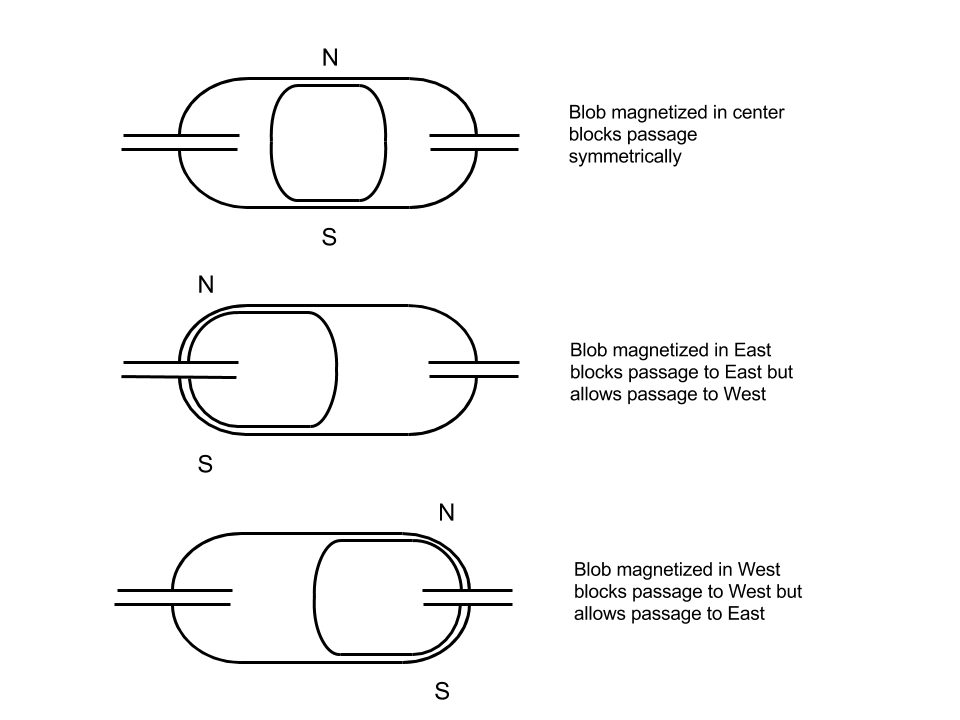
\includegraphics[width=1.0\textwidth]{BasicOperation.png}
%%      \caption{Basic Operation (Now considered incorrect!)}
%%   \label{fig:closeup}     
%% \end{figure}

\section{First Experiments}

Here is a simple experiment that any can do with ferrofluid, a petri dish, a magnet and a hypodermic syringe:
Place the ferrfluid in the dish. Cover it (to prevent splashes). Place a magnet beneath the ferrofluid.
Remove the cover.

You will now have a ``mound'' of ferrofluid.  Use the hypodermic needle to inject air into the mound.  You will
observe that the bubbles always flow down the magnetic gradient. That is, they always flow away from the volumes
of greater magnetic density.  This experiment can be made more interesting by placing several magnets below
the dish, to obtain a mound of ferrofluid which a magnetic field that drops to zero (where two oppose poles
meet.)

\section{Basic Experimental Apparatus}

At considerable trouble and without much success I have developed half-way working mechanisms of
performing experiments. In particular, I puchased a basic 1/8'' 100 psi pneumatics kit.

I quickly shifted to using ``column inches of water'' as a lower-pressure unit of measurement,
and to using a bike pump rather than an electric compressor.

My experimental set up consists of valves and gauges that let me create a measure pressure on
one side of my experiment valve.

I use hot-melt glue to attempt to seal the needles into clear plastic tubes.  I use rare-earth
magnets in the 1'' x 1/2'' cylindrical configuration to generate magnetic fields.

It is not clear that I have been able to make a completely leak proof system.

Originally, I use hypodermic syringes for this work.  However, these are so thin that they
support very little air flow and seem to clog easily.  I have since shifted to using the
needs used to inflate volleyballs and soccer balls, and am happier with that choice.
However, those needles are mounted to the plastic with hot-melt glue, a tedious and error-prone practice.

\section{Basic Results}

I have performed an experiment:

I create a ferrofluid blob between two pairs of two 1'' magnets (1/2'' diamter) (with attracing poles together)
inside the valve chamber.  Then I raise the high-side pressue to about 8 column-inches of water with the bicycle pump.
This pressure holds, losing aproximately 0.4 column-inches in one minute.  Then the magnets are withdrawn, the pressure
drops immediately.

I belive this proves the (very expected and unoriginal) result that you can create an air-tight plug of ferrofluid.
I do not know in this case if the slow loss in pressure is cause by a leak through the ferro-fluid plug or through
one of the joints in my system.

Proposed experiment to determine this:

If I manufacture a valve on the low side, I can anser this question by closing the valve.  We will be able
to determine if the whole system is air-tight or not.

\section{An Apparently Failing Experiment}

Using the same apparatus, when I move the magnet (and blob) to the point that the needle enters the blob,
passes the midpoint, and even extends past it, the pressure remains on the high-side.  I am quite surprised
by this; I expected the air to transfer as soon as the port of the needle moved past the mid-point.

If this is replicatable, it suggest that the ferrofluid in the needle is blocking the flow. This
seems to be in direct opposition to my theory.

It seems completely replcatable that if there is ferrofluid in the needle, then it forms a plug
that stops the flow.  This basically means my check valve doesn't work.

Okay, I have now repeated the experiment with a non-ferrous ``needle''.  It seems clear that the magnetized plug
does not let air pass as I expected it would.  I need to rethink this at a much more basic level.

\section{An enlightenment}

I now believe that I have been making a crucial mistake.  I can have been forcing the input manifold
to move throught the core of the blob. However, the intake manifold can enter on the side of the blob,
avoid the area of greatest density.

In this position, until the point where it breaks, we get one-wayness by requiing differing amounts of
work to go in different directions.  One direction has to move the whole blob, the other direction
has to move only a weakly interacting portion.  (Possibly this has a weakness in hydraulically pushing
more of the material away from the blob.)

\section{The Next Experimental Apparatus}


\begin{figure}
  \centering
     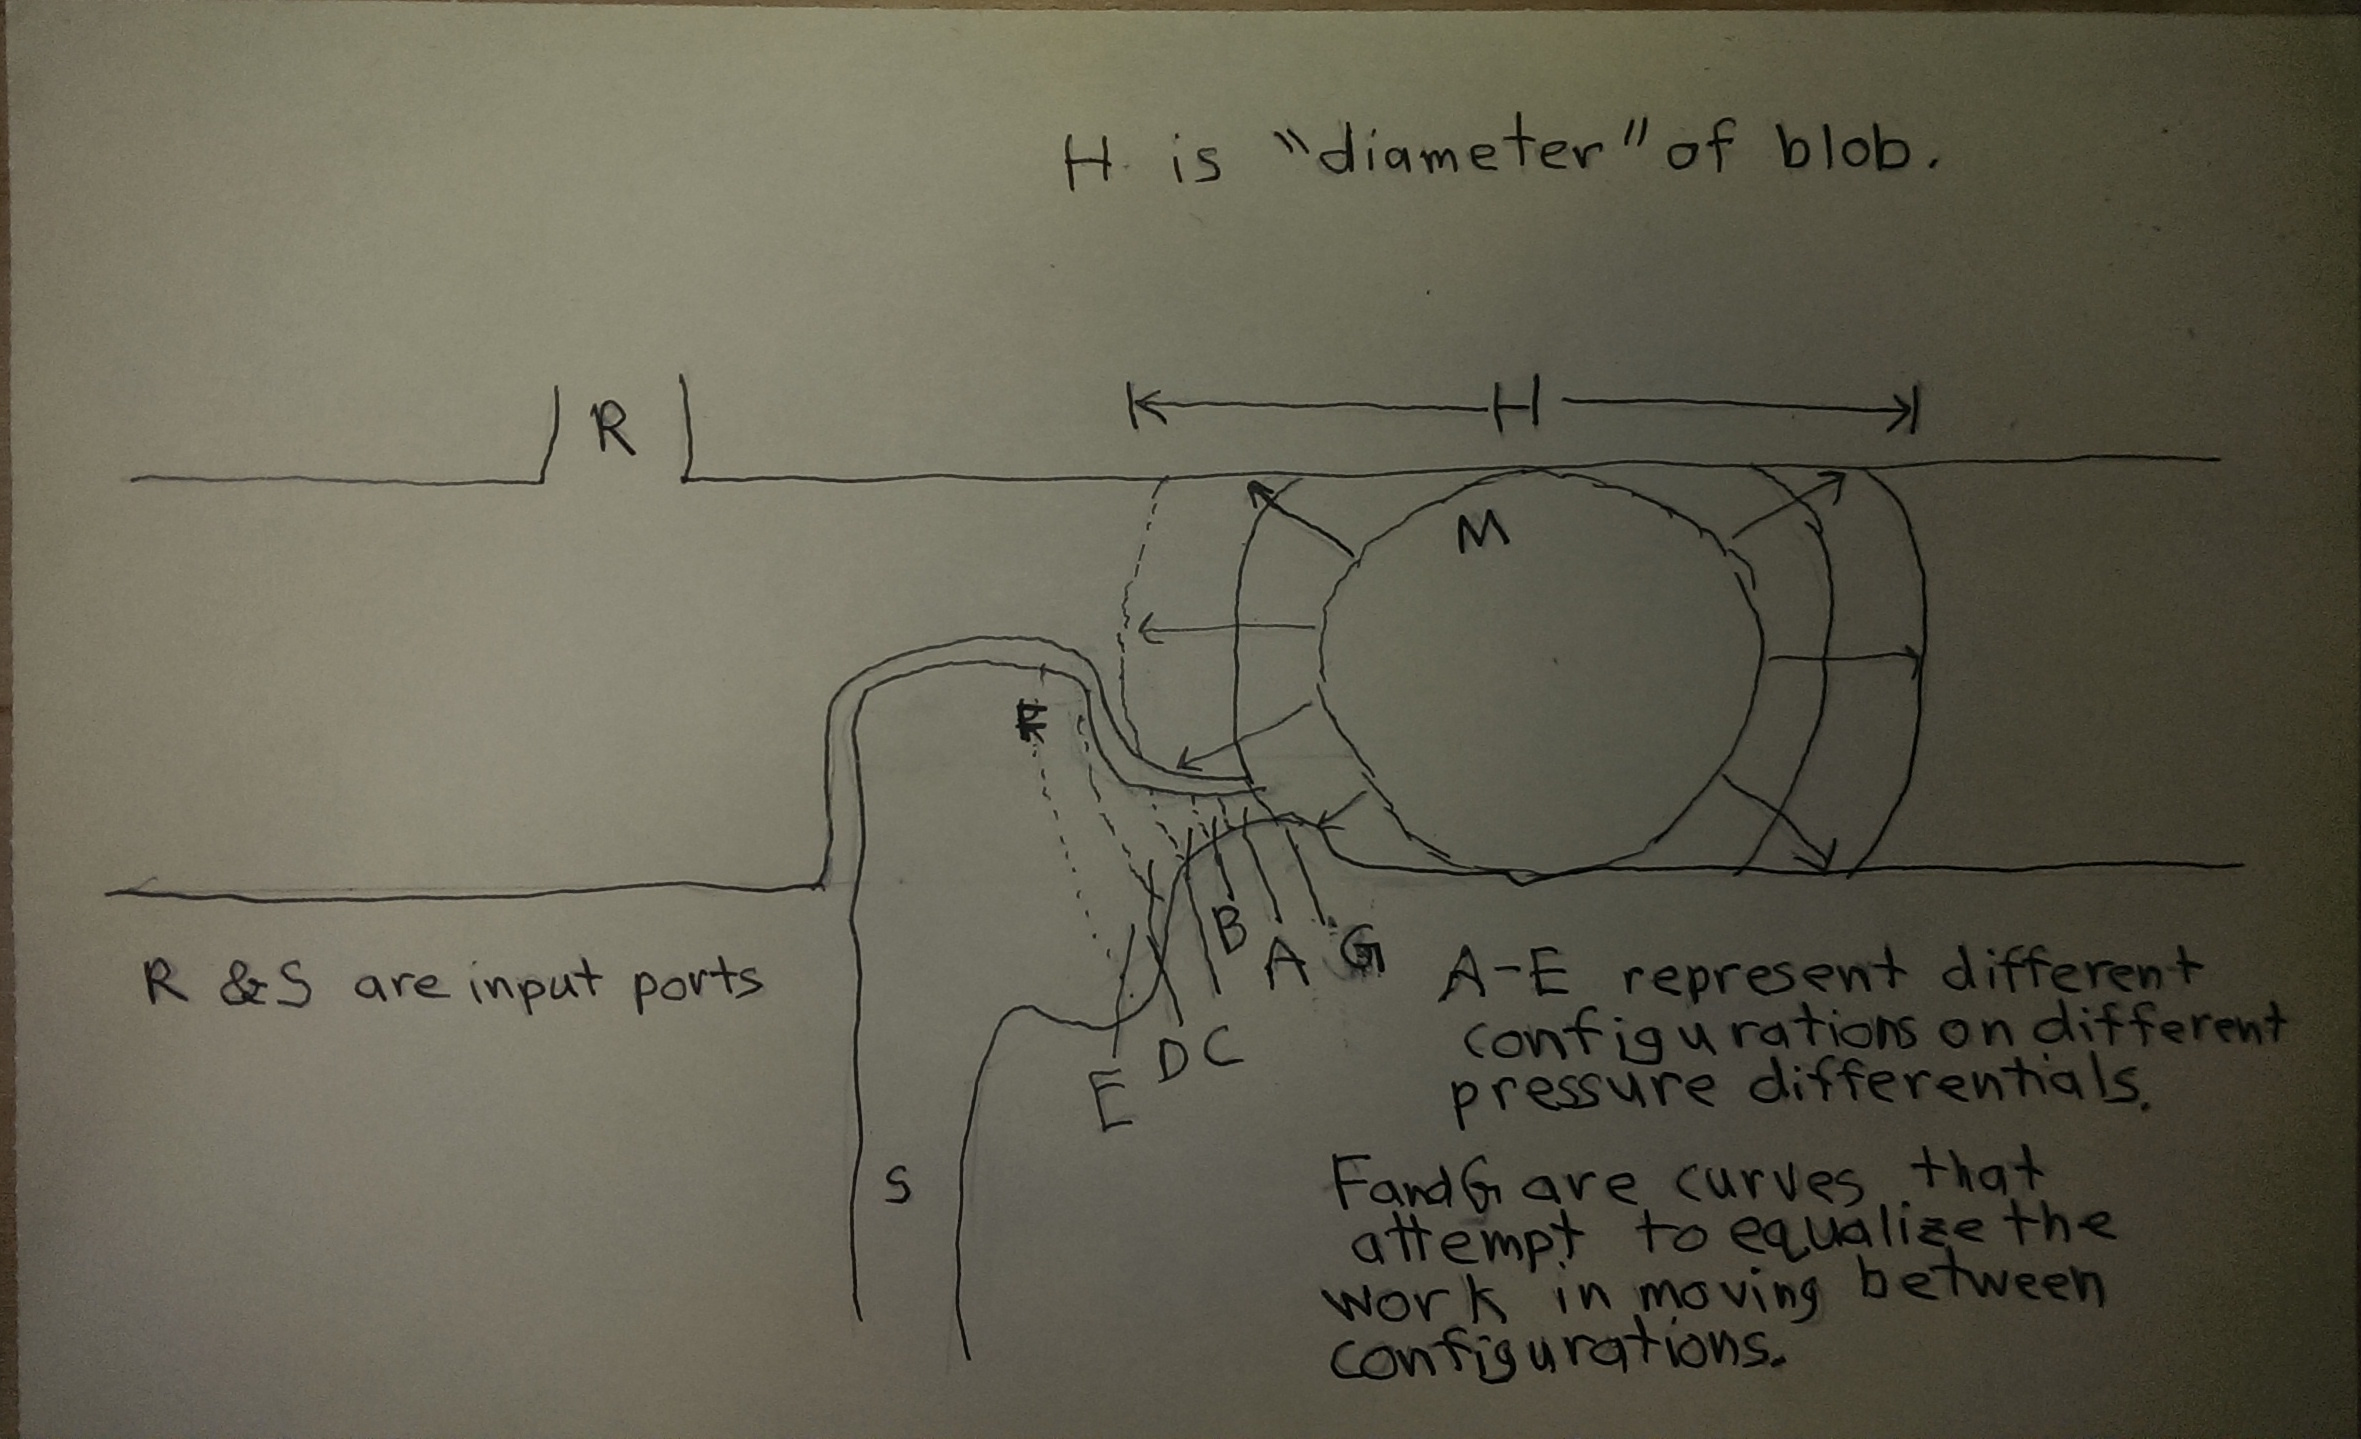
\includegraphics[width=1.0\textwidth]{CurvedInjection.jpg}
     \caption{Equiwork Injection Port}
  \label{fig:closeup}     
\end{figure}


\begin{figure}
  \centering
     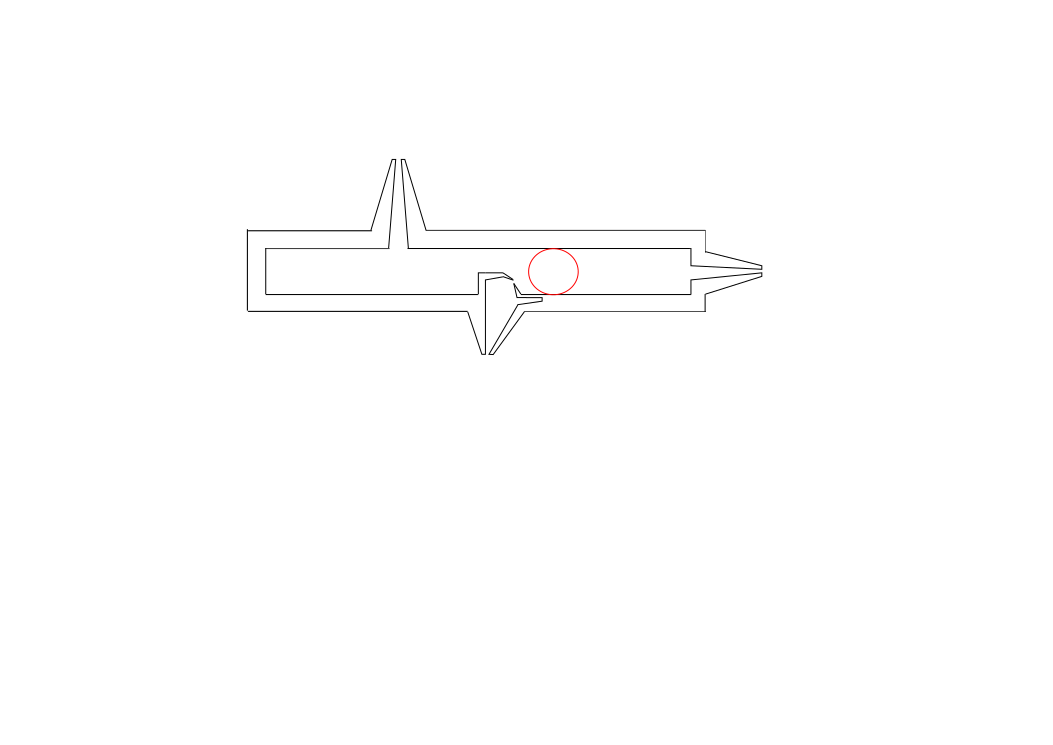
\includegraphics[width=1.0\textwidth]{designforlasercutting.png}
     \caption{Design For Laser Cutting}
  \label{fig:broadapparatus}     
\end{figure}

\begin{figure}
  \centering
     \includegraphics[width=1.0\textwidth]{thinpipeapparatus.png}
     \caption{Design For Laser Cutting}
  \label{fig:thinpipeapparatus}     
\end{figure}


I believe it is possible to improve what I am doing by having the the pass-through input port not go through the core of the magnetic
flux but enter fromt he side or front.

In fact, by making the port conical/triangular/horn shaped it should be possible to further establish the assymetry in pressure.
That is, in a triangle, pushing the ferrofluid out increase the area/volume that is near the magnetic field, while filling the
same space with air requires less and less work until the bubble pops out.


Let me attempt to explain some ideas with respect to \ref{fig:closeup}.
The figure is planar, but in fact represents a sandwich of three layers of acrylic, with chambers allows the containment of air
and ferrofluid.
\begin{itemize}
\item $M$ represents the projection of cylindrical magnets (one above and one below the sandwich.)
\item $H$ is meant to represent the general diameter of the blob, taken to be the longest measurable distance along
  the center of the chanmber.
\item $R$ and $S$ are twin input ports. As a check-valve, we want air to flow from $S$ to $R$, and not from $R$ to $S$.
\item $A..E$ represent distinct configurations representing different levels of pressure at $R$ and $S$.
  \item $F$ and $G$ are intended to be curves which attempt to demand equal work to move from one configuration to another.
  \end{itemize}

I would like to assert the following points:
\begin{itemize}
\item As the pressure $S$ increases relative to $R$, the ferrofluid moves through configuration $E$ to configuration $A$.
  \item If this pressure increase further still, a bubble will form which will move from $S$ into the ferrofluid blob.
    This bubble will then move into $R$ by virtue of the magnetic gradient.
  \item If we imagine magentic force increasing, the configuration will move toward $C$ (the configuration which has
    equidistant ferrofluid interfacing to $R$ and $S$.
  \item There are two curves $F$ and $G$ which are which eqalize the work needed to drive a system in equilibrium to
    a new equialibrium.
  \item The entire blob will move backward (away from $R$) as the pressure of $R$ is incresed.  At the same time,
    there will be pressure to move from (for example) $C$ to $D$.  However, the magnetic force will work against
    this, seeking to drive $D$ to $C$.
  \item Part of the purpose of the curves $F$ and $G$ is to increase the mass of that is acted upon by the magnetic
    force as the configuration increases. This assymmetry may be essential to the one-wayness of the valve.
  \end{itemize}

\section{Contact and Getting Involved}

Public Invention,
a free-libre, open-source research, hardware, and software project that welcomes volunteers.
To assist, contact:
\href{mailto:read.robert@gmail.com}{read.robert@gmail.com}.

\bibliographystyle{asmems4}
\bibliography{IEEEabrv,gluss}

\end{document}

https://infoscience.epfl.ch/record/55930/files/98.pdf

http://iris.elf.stuba.sk/jeeec/data/pdf/7s_110-41.pdf


